\chapter{L'eredità del terrore e i due piloti della mente}

\begin{flushright}
	\textit{``La paura è il prezzo che paghiamo per l'anticipazione.''}\\[6pt]
	\textsc{Joseph LeDoux}
\end{flushright}

\bigskip

\section{L'eredità del terrore}

Centomila anni fa, nella savana africana. Il sole sta tramontando. Un nostro antenato si è allontanato dal gruppo per raccogliere radici. Improvvisamente, un fruscio nell'erba alta. Potrebbe essere il vento. Potrebbe essere una preda in fuga. Potrebbe essere un leopardo in agguato. Ha una frazione di secondo per decidere, e in quella frazione di secondo si gioca tutto.

Chi si fermava ad analizzare razionalmente la situazione, valutando la direzione del vento, l'altezza dell'erba, la probabilità statistica di trovare predatori in quella zona, non ha lasciato discendenti. Chi saltava e correva al primo rumore sospetto ha tramandato i suoi geni. E con quei geni ha tramandato un sistema di allarme calibrato su un principio tanto brutale quanto efficace: meglio mille spaventi inutili che una sola morte evitabile.\footnote{Marks, I. M., e Nesse, R. M. (1994). Fear and fitness: An evolutionary analysis of anxiety disorders. \textit{Ethology and Sociobiology}, 15(5).}

Quel sistema di allarme ancestrale vive ancora oggi dentro di voi, perfettamente intatto. Solo che adesso non reagisce più ai fruscii nella savana, ma alle vibrazioni del telefono sul comodino, al tono di voce del capo durante una riunione, ai titoli allarmistici che scorrono sullo schermo. Il corpo si prepara a combattere o a fuggire di fronte a minacce che non richiedono né l'una né l'altra cosa: una email, una notifica, un messaggio visualizzato e rimasto senza risposta.\footnote{Sapolsky, R. M. (2004). \textit{Why Zebras Don't Get Ulcers}. Times Books, New York.}

\begin{center}
	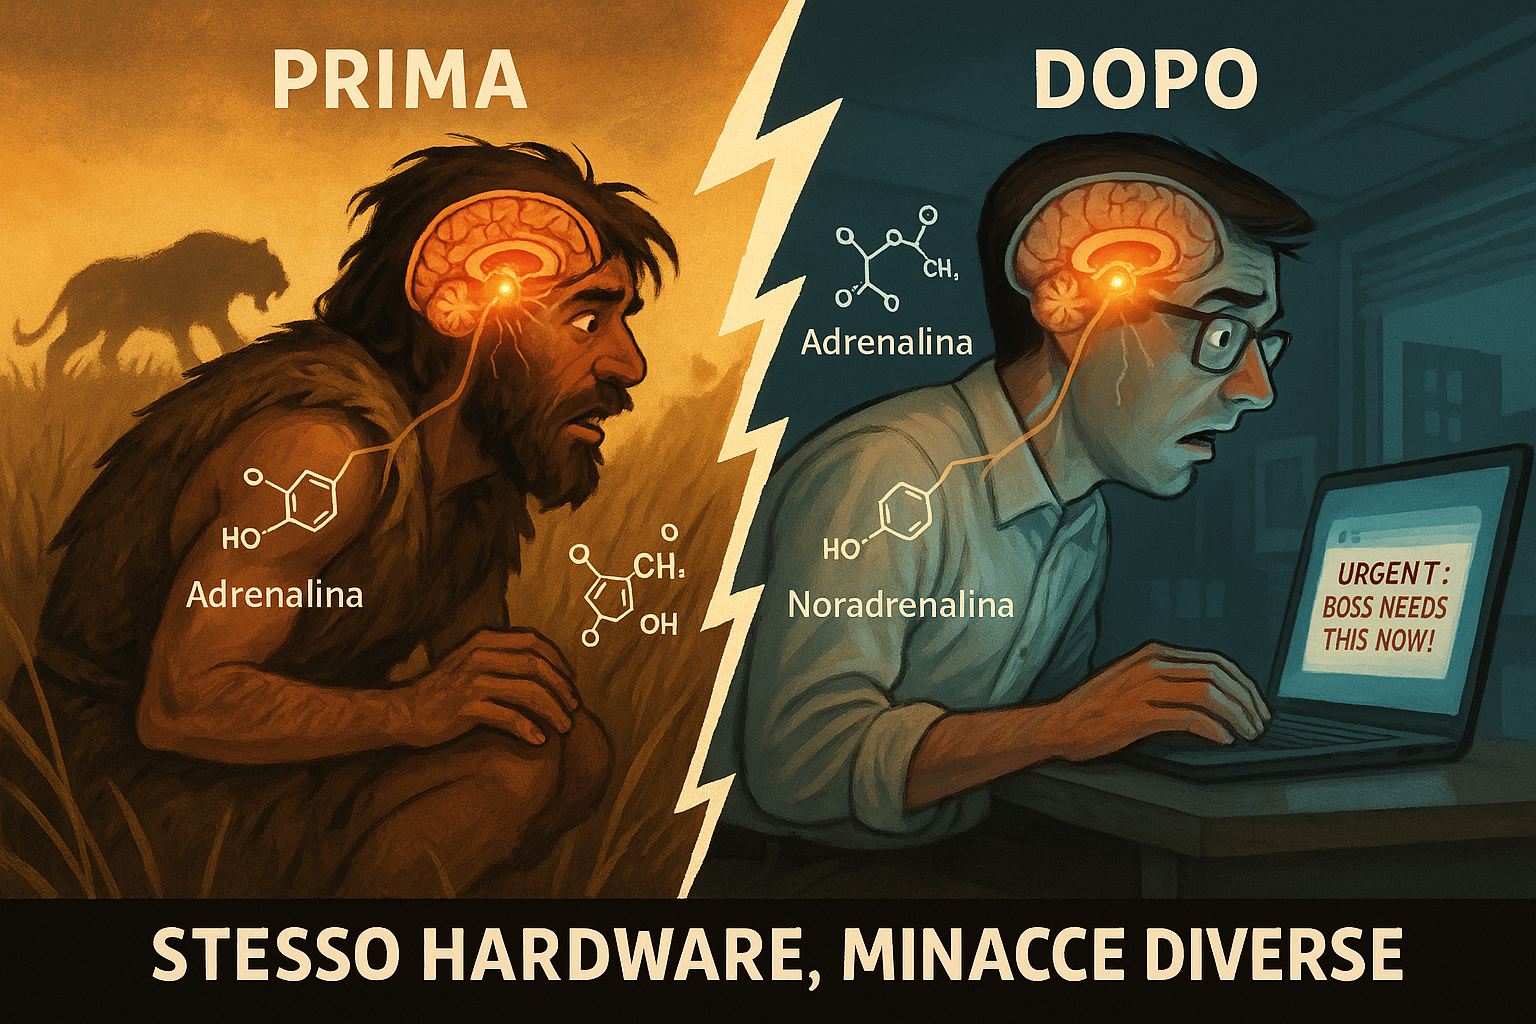
\includegraphics[width=1\textwidth]{images/prima_dopo2.png}
	\captionof{figure}{Stesso hardware biologico, minacce completamente diverse. Il sistema che rilasciava adrenalina per sfuggire a un predatore ora rilascia cortisolo per una email urgente. L'evoluzione non ha avuto il tempo di aggiornarsi.}
	\label{fig:stress_evolution}
\end{center}

Al centro di questo meccanismo c'è una piccola struttura a forma di mandorla, sepolta in profondità nei due emisferi: \index[main]{amigdala}\textbf{l'amigdala}. È la sentinella più antica e più nervosa del nostro cervello, la guardia notturna che non dorme mai e che ha un solo compito, decidere in pochi millisecondi se ciò che accade fuori è una minaccia. Quando crede di averne trovata una, non chiede il permesso a nessuno: tira la leva dell'allarme e inonda l'intero organismo di ormoni dello stress, prima ancora che la parte pensante del cervello abbia avuto il tempo di farsi un'opinione.

Qui sorge una domanda che la scienza moderna pone con i suoi strumenti, ma che un filosofo aveva già posto con la sola forza del pensiero quasi quattro secoli fa. Siamo abituati a considerare la paura, la rabbia, il desiderio come difetti, come momenti in cui smettiamo di essere noi stessi. Eppure, se queste passioni sono scritte nella nostra biologia da centinaia di milioni di anni, possono davvero essere dei semplici errori?

A questa domanda rispose Baruch Spinoza, un pensatore olandese del Seicento che lavorava di giorno levigando lenti per microscopi e di notte costruendo uno dei sistemi filosofici più ambiziosi della storia. Nella sua opera maggiore, l'\textit{Etica}, scritta in forma di teoremi geometrici come fosse un trattato di matematica, Spinoza sostenne qualcosa di rivoluzionario: \textbf{le passioni non sono guasti della ragione, sono forze della natura}.\footnote{Spinoza, B. (1677). \textit{Ethica, ordine geometrico demonstrata}. Pubblicazione postuma, Amsterdam.} Pretendere di eliminarle è assurdo come pretendere di proibire a un sasso di cadere. Il compito della ragione non è reprimerle, ma comprenderle.

Al cuore di questa visione c'è un concetto che suona stranamente familiare a chiunque abbia studiato un poco di biologia: il \textit{conatus}, lo sforzo con cui ogni essere tende a perseverare nella propria esistenza. Per Spinoza, ogni cosa viva è attraversata da questa spinta cieca e potente a conservarsi, a difendersi, a continuare a esistere. È la stessa identica forza che, milioni di anni più tardi, i neuroscienziati ritroveranno nell'amigdala che scatta al fruscio nell'erba. Spinoza, senza avere mai visto un cervello sotto un microscopio, aveva intuito che dentro di noi opera un motore di autoconservazione che precede ogni ragionamento. Aveva descritto, in linguaggio filosofico, ciò che oggi chiamiamo il nostro sistema di sopravvivenza più antico.

\begin{figure}[htbp]
	\centering
	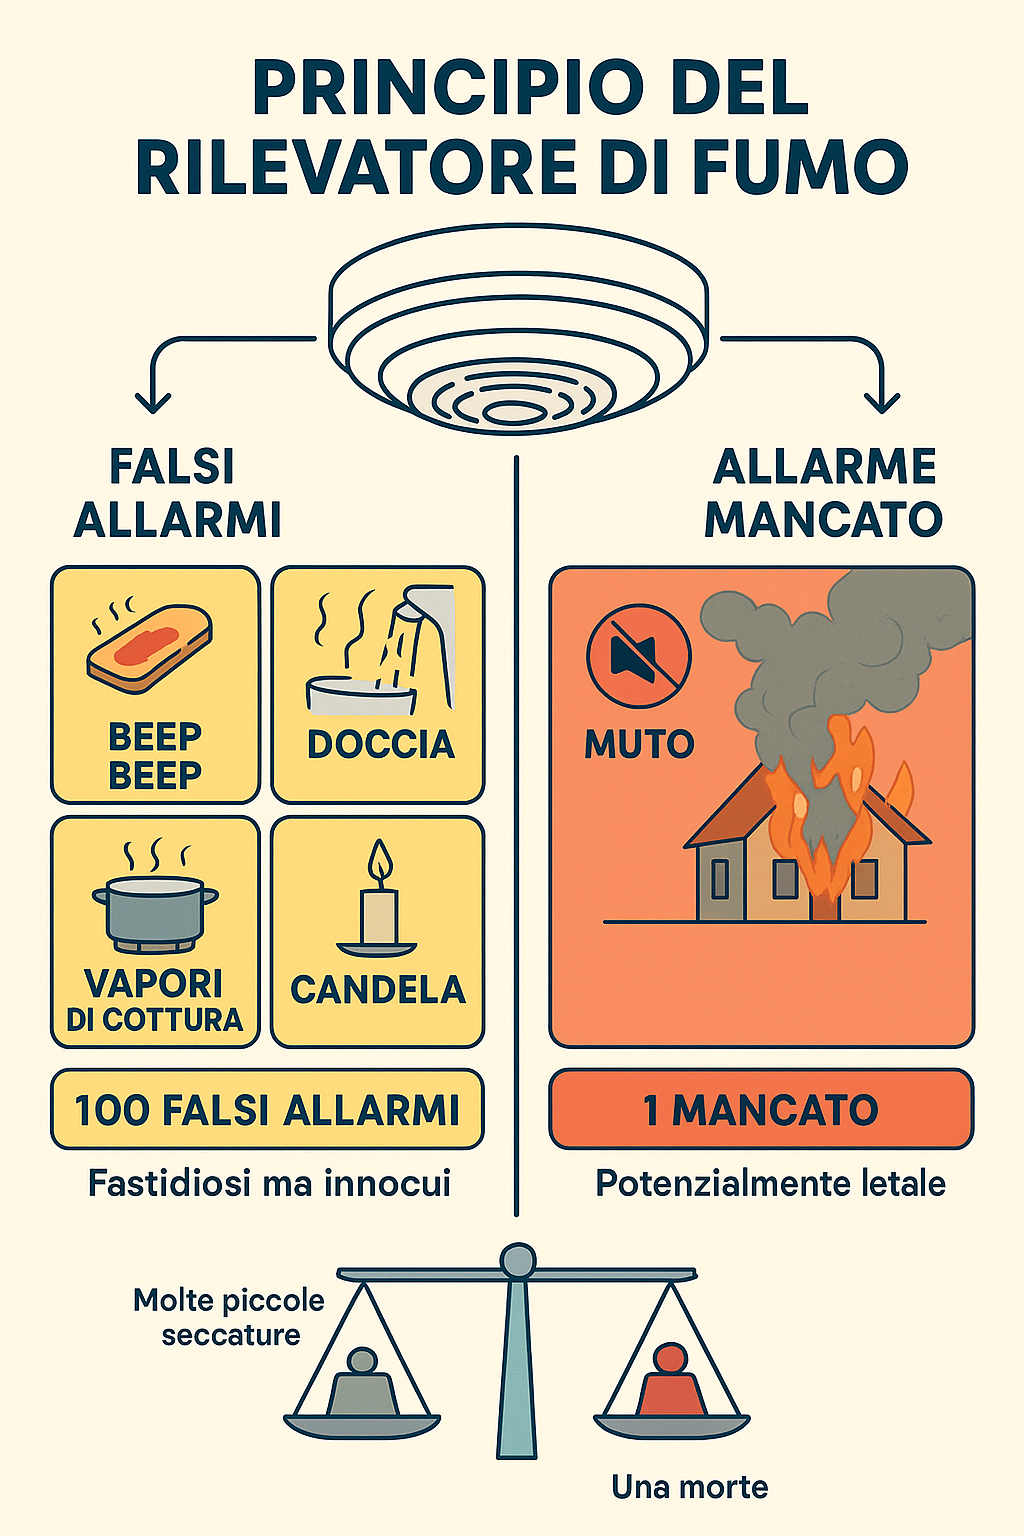
\includegraphics[width=0.9\textwidth]{images/bilancia_allarmi.png}
	\captionof{figure}{Meglio cento spaventi inutili che una sola morte evitabile: il cervello preferisce reagire troppo piuttosto che troppo poco. È la logica evolutiva che ci tiene in vita da millenni.}
	\label{fig:smoke_detector}
\end{figure}

\index[main]{Nesse, Randy}Randy Nesse ha mostrato che tutta questa logica ancestrale segue un principio di una semplicità elegante, quello che lui chiama il \textit{principio del rilevatore di fumo}.\footnote{Nesse, R. M. (2005). Natural selection and the regulation of defenses: A signal detection analysis of the smoke detector principle. \textit{Evolution and Human Behavior}, 26(1).} Un allarme antincendio che suona dieci volte per una fetta di pane bruciacchiata è fastidioso ma utile. Un allarme che resta in silenzio durante un vero incendio è fatale. Conviene dunque tarare il sistema sulla iperreazione: meglio cento falsi allarmi che una sola tragedia mancata.



Lo si osserva con chiarezza disarmante in un genitore con il primo figlio. Ogni colpo di tosse diventa una possibile polmonite, ogni caduta una potenziale commozione, ogni linea di febbre una emergenza pediatrica. Gli altri genitori sorridono con indulgenza, perché sanno che al terzo figlio controllerai a malapena se respira ancora. Eppure il meccanismo è perfetto proprio nella sua apparente irrazionalità: meglio dieci corse inutili al pronto soccorso che mancare l'unica volta in cui c'era davvero qualcosa che non andava. Lo stesso vale per il sistema immunitario, che scatena l'inferno delle allergie contro un granello di polline innocuo, perché quella stessa ipersensibilità è ciò che lo rende pronto contro un virus che potrebbe ucciderci.


Il problema è che oggi quel genitore iperprotettivo che abbiamo in testa scambia una email del capo per una tigre dai denti a sciabola. E a differenza dei genitori veri, che con il tempo imparano a rilassarsi, il nostro sistema di allarme non ha mai imparato che certe minacce erano soltanto per finta.\footnote{Haselton, M. G., e Nettle, D. (2006). The paranoid optimist: An integrative evolutionary model of cognitive biases. \textit{Personality and Social Psychology Review}, 10(1).}

\section{I due piloti e la ragione serva delle passioni}

A questo punto i ricercatori hanno fatto qualcosa di affascinante: hanno cronometrato la gara. Hanno applicato elettrodi sulla testa di volontari e misurato, millesimo di secondo dopo millesimo di secondo, cosa accade nel cervello quando compare un pericolo. I risultati sono insieme rassicuranti e inquietanti.

Quando il sistema rileva una minaccia, l'amigdala si attiva in dodici, venti millisecondi.\footnote{LeDoux, J. (1996). \textit{The Emotional Brain}. Simon and Schuster, New York.} La corteccia prefrontale, la parte saggia del cervello che potrebbe sussurrare ``calma, è solo una email'', impiega almeno duecentocinquanta millisecondi per entrare in scena.\footnote{Bar, M., e altri (2006). Top down facilitation of visual recognition. \textit{PNAS}, 103(2).} Per un quarto di secondo, siamo letteralmente in balia della reazione primitiva. È come se due piloti si contendessero lo stesso volante, ma uno dei due avesse sempre il controllo esclusivo nei primi metri di ogni curva.

\begin{figure}[htbp]
	\centering
	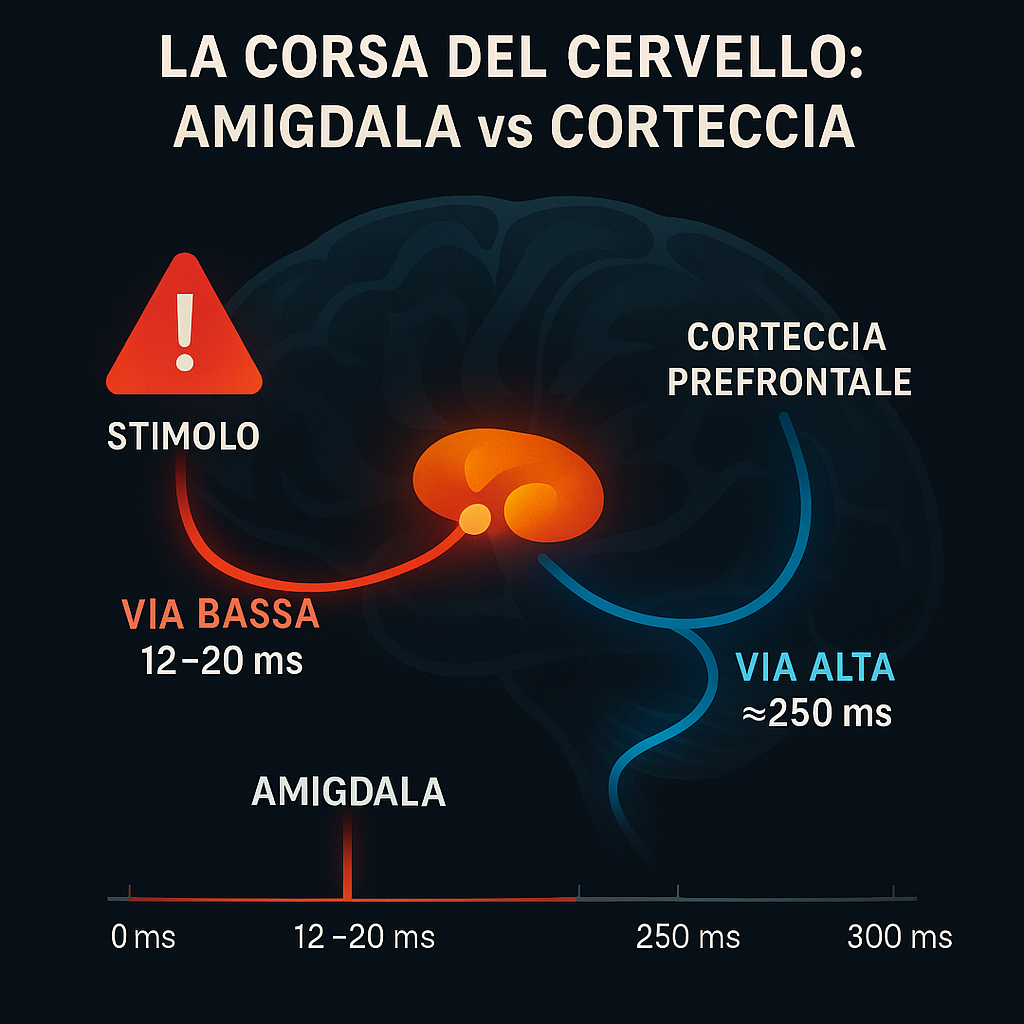
\includegraphics[width=0.8\textwidth]{images/tempi_amigdala.png}
	\caption{La gara persa in partenza. L'amigdala reagisce in dodici, venti millisecondi mentre la corteccia prefrontale ne richiede almeno duecentocinquanta, creando una finestra temporale in cui siamo governati dall'istinto puro.}
	\label{fig:funzionamento_amigdala}
\end{figure}

Abbiamo già incontrato questi due piloti nelle pagine precedenti: il Sistema 1, veloce, automatico, emotivo, antico, e il Sistema 2, lento, deliberato, razionale, costoso da mantenere acceso.\footnote{Kahneman, D. (2011). \textit{Thinking, Fast and Slow}. Farrar, Straus and Giroux, New York.} La gara cronometrata in laboratorio non fa che misurare, al millisecondo, una verità che già sospettavamo: il pilota emotivo parte sempre per primo. E quando il Sistema 2 finalmente arriva, spesso non trova una decisione da prendere, ma una decisione già presa, che gli viene solo chiesto di approvare. Gli psicologi lo chiamano \index[main]{ragionamento motivato}ragionamento motivato: non usiamo l'analisi razionale per scoprire la verità, ma per giustificare ciò che già sentivamo.\footnote{Kunda, Z. (1990). The case for motivated reasoning. \textit{Psychological Bulletin}, 108(3).} Il Sistema 2 diventa l'avvocato del Sistema 1, non il suo giudice.

Se questa idea vi sembra una scoperta recente delle neuroscienze, preparatevi a una sorpresa. Nel 1739, un giovanissimo filosofo scozzese di nome David Hume pubblicò un'opera che le librerie del tempo ignorarono quasi completamente, il \textit{Trattato sulla natura umana}. Conteneva una frase destinata a diventare una delle più scandalose e profetiche della storia del pensiero: \textit{la ragione è, e deve soltanto essere, schiava delle passioni}.\footnote{Hume, D. (1739). \textit{A Treatise of Human Nature}. John Noon, Londra.}

Provate a immaginare lo scandalo. Per secoli la filosofia aveva celebrato la ragione come il cocchiere che doveva tenere a freno i cavalli, la regina che governava il regno disordinato delle emozioni. Hume capovolge tutto. Sostiene che la ragione, da sola, non muove un dito. Può calcolare conseguenze, confrontare mezzi e fini, illuminare la strada. Ma il movimento, la spinta, la decisione di partire, quelle vengono dal desiderio, dalla paura, dall'attaccamento. La ragione tiene la mappa, ma è la passione che decide la destinazione e mette in moto i cavalli.

Per quasi due secoli questa fu considerata una provocazione brillante ma eccessiva. Poi arrivarono gli elettrodi, le risonanze magnetiche, i cronometri che misurano i millisecondi. E si scoprì che Hume aveva ragione in un senso quasi imbarazzantemente letterale. Il Sistema 1 emotivo parte davvero prima del Sistema 2 razionale. La passione precede davvero la ragione, non in senso poetico, ma in senso cronologico, misurabile, fotografabile dentro un cervello. Un filosofo seduto alla sua scrivania a Edimburgo, senza alcuno strumento se non l'osservazione di se stesso, aveva anticipato di duecento anni ciò che la tecnologia avrebbe dovuto faticare per dimostrare.

\section{La fabbrica delle emozioni}

L'amigdala e il suo allarme, però, sono solo la punta dell'iceberg. Il cervello è una vera e propria fabbrica di emozioni, con reparti specializzati, catene di montaggio e un controllo qualità che ogni tanto si inceppa. È un'operazione industriale su scala neuronale, con milioni di cellule che lavorano senza sosta per produrre quella miscela chimica che chiamiamo sentimenti.

Il guaio è che questa fabbrica fu progettata milioni di anni fa per un catalogo molto ristretto, paura, rabbia, gioia, tristezza, disgusto, sorpresa, ma oggi deve evadere ordini infinitamente più complessi: ansia da prestazione, invidia da social network, paura di restare esclusi, esaurimento da lavoro, crisi esistenziali.\footnote{Barrett, L. F. (2017). \textit{How Emotions Are Made: The Secret Life of the Brain}. Houghton Mifflin Harcourt, Boston.} È come chiedere a una fabbrica di candele dell'Ottocento di assemblare smartphone: tecnicamente si tratta sempre di mettere insieme dei pezzi, ma la complessità è esplosa mentre i macchinari sono rimasti gli stessi.

E qui dobbiamo fermarci su una domanda che sembra ingenua e invece è abissale. Quando provate paura, cosa viene prima? Il sentimento o il battito accelerato? La tristezza o le lacrime? La risposta ovvia sarebbe: prima sento, poi il corpo reagisce. Prima ho paura, poi tremo. Prima sono triste, poi piango.

Alla fine dell'Ottocento, uno dei padri della psicologia moderna ribaltò anche questa certezza. William James, fratello del romanziere Henry, propose una tesi che a prima vista sembra una follia: \textit{noi non tremiamo perché abbiamo paura, abbiamo paura perché tremiamo. Non piangiamo perché siamo tristi, siamo tristi perché piangiamo.}\footnote{James, W. (1890). \textit{The Principles of Psychology}. Henry Holt and Company, New York.} Secondo James, ciò che chiamiamo emozione non è altro che la percezione di ciò che sta accadendo nel nostro corpo. Prima il corpo si attiva, il cuore accelera, i muscoli si tendono, lo stomaco si chiude. Poi il cervello legge questi segnali e li traduce in un'etichetta: ``ho paura''.

Per decenni questa idea fu archiviata come una curiosità un po' bizzarra. Finché, alla fine del Novecento, un neuroscienziato di nome \textbf{Antonio Damasio} non la riportò in vita con prove cliniche. Studiando pazienti che, a causa di specifiche lesioni cerebrali, avevano perso la capacità di provare emozioni pur conservando un'intelligenza intatta, Damasio scoprì che queste persone, perfettamente capaci di ragionare, erano diventate incapaci di decidere. Davanti alla scelta più banale restavano paralizzate, soppesando all'infinito i pro e i contro senza mai arrivare a una conclusione. Da qui la sua ipotesi del \textit{marcatore somatico}: il corpo emette segnali, una stretta allo stomaco, un senso di sollievo, e sono questi segnali corporei a guidare le nostre scelte ben prima che la ragione li traduca in parole.\footnote{Damasio, A. R. (1994). \textit{Descartes' Error: Emotion, Reason, and the Human Brain}. Putnam, New York.} James aveva visto giusto un secolo prima: l'emozione nasce nel corpo, e la mente arriva dopo a leggerla.

Questa fabbrica produce alcuni modelli con una facilità sospetta. \index[main]{Seligman, Martin}Martin Seligman ha mostrato che possediamo paure preparate, predisposizioni biologiche verso certi pericoli.\footnote{Seligman, M. E. (1971). Phobias and preparedness. \textit{Behavior Therapy}, 2(3).} Il nostro kit di serie include serpenti, ragni, altezze, spazi chiusi, sangue, estranei, isolamento. Notate cosa manca: niente automobili, che pure uccidono migliaia di persone ogni anno, niente prese elettriche, niente armi da fuoco. Il catalogo è rimasto fermo al Pleistocene. E basta una sola esperienza negativa per installare una paura permanente: un morso da bambino, e la paura dei cani resta per la vita. Il cervello applica due pesi e due misure: una sola prova gli basta per certificare un pericolo, infinite prove non gli bastano mai per certificare la sicurezza.\footnote{Öhman, A., e Mineka, S. (2001). Fears, phobias, and preparedness: Toward an evolved module of fear and fear learning. \textit{Psychological Review}, 108(3).}

C'è poi un altro reparto, quello della ricompensa, il celebre circuito dopaminergico. Il suo motto aziendale potrebbe essere: se ti fa stare bene, allora deve essere importante per la sopravvivenza.\footnote{Schultz, W. (2015). Neuronal reward and decision signals: From theories to data. \textit{Physiological Reviews}, 95(3).} Nella versione originale funzionava a meraviglia. Cibo, dopamina. Una fonte d'acqua, dopamina. Un successo sociale, dopamina. Ciò che faceva stare bene era quasi sempre ciò che aumentava le probabilità di sopravvivere. Poi sono arrivati il gioco d'azzardo, i social, il cibo ultraprocessato, lo shopping con un clic, e hanno scoperto la combinazione della cassaforte. Tutte cose che azionano la leva della ricompensa senza avere nulla a che fare con la sopravvivenza.\footnote{Volkow, N. D., Wang, G. J., Fowler, J. S., e Telang, F. (2008). Overlapping neuronal circuits in addiction and obesity. \textit{Philosophical Transactions of the Royal Society B}, 363(1507).} È come se qualcuno avesse violato il software della fabbrica. Il cervello continua a insistere: questo schermo deve essere importante per la tua sopravvivenza, altrimenti perché ti darebbe tanta soddisfazione?

Il prodotto più sorprendente di questa fabbrica è la sofisticazione che si nasconde dietro emozioni apparentemente semplici. Prendete la \index[main]{gelosia}gelosia. Sembra un sentimento unico, monolitico. In realtà è un cocktail di almeno sei ingredienti distinti: paura dell'abbandono, rabbia per la perdita di controllo, ansia per l'incertezza, tristezza per la perdita percepita, invidia per ciò che l'altro possiede, e perfino una punta di disgusto morale.\footnote{Harmon Jones, E., Peterson, C. K., e Harris, C. R. (2009). Jealousy: Novel methods and neural correlates. \textit{Emotion}, 9(1).} Questi ingredienti vengono dosati in proporzioni diverse a seconda della situazione, della persona, perfino dell'ora del giorno. E tutto avviene in pochi millisecondi, senza alcuna supervisione cosciente. Quando James diceva che l'emozione è la lettura di uno stato del corpo, intendeva proprio questo: ciò che sentiamo come un blocco unico è in verità un'orchestra di segnali corporei che il cervello compone in tempo reale.

\section{Il tutore severo: quando l'errore diventa maestro}

C'è un reparto di questa fabbrica che merita attenzione speciale, perché produce qualcosa che a prima vista sembra crudele e che invece è uno dei capolavori del nostro funzionamento: \textit{il disagio educativo}. Il cervello ha imparato a trasformare gli errori in lezioni indimenticabili attraverso una dose calibrata di sofferenza.

Quando sbagliate, che sia prendere la strada sbagliata o investire i risparmi nella startup di un amico che prometteva di rivoluzionare il mercato dei calzini intelligenti, accade qualcosa di preciso nel cervello. Entro cinquanta, cento millisecondi, una regione chiamata corteccia cingolata anteriore produce un segnale elettrico che i neuroscienziati hanno battezzato \index[main]{error related negativity}negatività correlata all'errore: in sostanza un campanello che dice ``attenzione, qualcosa è andato storto, ricordatelo bene''.\footnote{Holroyd, C. B., e Coles, M. G. (2002). The neural basis of human error processing: reinforcement learning, dopamine, and the error related negativity. \textit{Psychological Review}, 109(4).} Il fastidio che provate nell'accorgervi dello sbaglio non è un effetto collaterale spiacevole: è il sistema che funziona alla perfezione. La parte più antica di voi non si fida dei ragionamenti astratti, ha bisogno che la lezione sia accompagnata da una sensazione viscerale, qualcosa che il corpo possa ricordare. Il dolore emotivo dell'errore è un evidenziatore biologico che marca l'esperienza come da non ripetere.

\index[main]{Schultz, Wolfram}Wolfram Schultz ha individuato il meccanismo preciso studiando i neuroni della dopamina.\footnote{Schultz, W. (2015). Neuronal reward and decision signals: From theories to data. \textit{Physiological Reviews}, 95(3).} Questi neuroni non si limitano a festeggiare le ricompense: tengono una contabilità continua tra ciò che ci aspettavamo e ciò che accade davvero. Quando le cose vanno meglio del previsto, sprigionano dopamina. Quando vanno peggio, la tagliano di colpo. E questa oscillazione modifica fisicamente le connessioni tra i neuroni, riscrivendo il cablaggio del cervello per affinare le previsioni future. È un sistema di apprendimento straordinariamente efficiente, ma ha un prezzo: il cortisolo liberato durante il disagio non si limita a farci stare male, amplifica in modo selettivo la formazione di quel ricordo.\footnote{McGaugh, J. L. (2018). Emotional arousal regulation of memory consolidation. \textit{Current Opinion in Behavioral Sciences}, 19.} Ecco perché ricordate con nitidezza l'imbarazzo di aver chiamato ``mamma'' la maestra alle elementari, ma avete dimenticato cosa avete mangiato lo scorso martedì. Le memorie cariche di emozione, soprattutto quelle spiacevoli, godono di un trattamento di favore nell'archivio.

Qui ritorna in scena la lezione di Spinoza. Quel disagio che ci insegna a non ripetere l'errore non è la ragione che corregge la passione, è una passione, la sofferenza, che educa il comportamento. La natura non ci ha dotati di un freddo calcolatore degli sbagli, ci ha dotati di un corpo che soffre e proprio per questo impara. Si capisce così perché impariamo molto più dagli errori che dai successi: il successo rilascia dopamina e ci fa sentire bene, ma non crea la stessa urgenza nella memoria. Il cervello archivia il successo come ``tutto regolare, prosegui''. L'errore, invece, scatena una tempesta di cortisolo, dopamina in caduta, amigdala in allerta, memoria potenziata.

Questo meccanismo, però, ha un lato oscuro. In alcune persone il tutore interno diventa così severo che il disagio dell'errore paralizza invece di insegnare. È la differenza tra dire ``ho commesso un errore, cosa posso imparare?'' e dire ``sono una persona che fa errori, sono un fallimento''. Il primo usa il sistema come è stato progettato. Il secondo resta intrappolato nel cortisolo senza mai arrivare alla lezione.

\section{Quando il sistema va in tilt}

Come ogni fabbrica, anche quella emotiva ha i suoi difetti di produzione. Il primo è la cosiddetta \index[cognitive]{euristica dell'affetto}euristica dell'affetto, la tendenza a giudicare situazioni complesse in base a come ci fanno sentire, anziché a un'analisi dei fatti.\footnote{Slovic, P., Finucane, M. L., Peters, E., e MacGregor, D. G. (2007). The affect heuristic. \textit{European Journal of Operational Research}, 177(3).} Un investimento vi ``sembra'' buono? Allora dev'essere buono. Una persona vi dà una ``brutta sensazione''? Allora dev'essere cattiva.

C'è poi un effetto curioso: la fabbrica produce emozioni che si autoconfermano. Avete notato come, quando siete già di cattivo umore, tutto sembra andare storto? Non è il mondo a essere diventato improvvisamente ostile, è la vostra fabbrica, regolata su ``modalità negativa'', che inizia a interpretare in chiave negativa anche eventi del tutto neutri.\footnote{Bower, G. H. (1981). Mood and memory. \textit{American Psychologist}, 36(2).} Il collega che non vi saluta? Ce l'ha con voi. Il commesso un po' brusco? Vi ha preso di mira. È il pregiudizio di conferma applicato ai sentimenti: non solo cerchiamo informazioni che confermano ciò che pensiamo, ma produciamo emozioni che confermano ciò che sentiamo.

Il difetto più pericoloso, però, è il sequestro emotivo. È ciò che accade quando l'amigdala dichiara lo stato di emergenza e si impossessa dell'intera operazione.\footnote{Goleman, D. (1995). \textit{Emotional Intelligence}. Bantam Books, New York.} In quei momenti la fabbrica smette di produrre la consueta gamma equilibrata di sensazioni e sforna quantità massicce di una sola emozione, di solito rabbia o paura. Siete ``troppo arrabbiati per pensare'', ``troppo spaventati per ragionare''. La parte logica del cervello è andata letteralmente fuori linea. Aveva un senso quando le emergenze erano leoni in caccia. Oggi le nostre emergenze sono messaggi del capo e commenti acidi sotto un post.

Ed è qui che emerge il paradosso più inquietante: viviamo, oggettivamente, nell'epoca più sicura della storia umana. \index[main]{Pinker, Steven}Steven Pinker ha documentato il declino drastico di quasi ogni forma di violenza.\footnote{Pinker, S. (2011). \textit{The Better Angels of Our Nature: Why Violence Has Declined}. Viking, New York.} Eppure i disturbi d'ansia colpiscono un italiano su quattro nel corso della vita,\footnote{de Girolamo, G., e altri (2006). Prevalence of common mental disorders in Italy. \textit{Social Psychiatry and Psychiatric Epidemiology}, 41(11).} e il consumo di ansiolitici nel Paese è raddoppiato in vent'anni.\footnote{Rapporto OsMed (2023). \textit{L'uso dei farmaci in Italia}. Agenzia Italiana del Farmaco, Roma.} \index[main]{Ropeik, David}David Ropeik suggerisce che non si tratta di una contraddizione, ma di una conseguenza diretta.\footnote{Ropeik, D. (2010). \textit{How Risky Is It, Really?}. McGraw Hill, New York.} In assenza di tigri reali, il sistema di allarme abbassa la soglia e comincia a reagire a tigri sempre più metaforiche. Nel mondo dei nostri antenati le minacce comparivano e svanivano. Oggi sono croniche: il flusso di notizie negative non finisce mai, i social erogano allarmi a ogni ora, la email ansiogena resta nella casella come un predatore che non se ne va più.\footnote{McEwen, B. S. (2017). Neurobiological and systemic effects of chronic stress. \textit{Chronic Stress}, 1.}

La situazione precipita quando il pilota razionale è stanco. Alcuni studi mostrano che i giudici affaticati emettono sentenze più severe,\footnote{Danziger, S., Levav, J., e Avnaim Pesso, L. (2011). Extraneous factors in judicial decisions. \textit{Proceedings of the National Academy of Sciences}, 108(17).} che i medici esausti commettono più errori diagnostici, che i dirigenti sovraccarichi prendono decisioni più rischiose. Non diventano stupidi: semplicemente il loro Sistema 2 è troppo provato per lavorare, e il Sistema 1 prende il comando assoluto.

Arriviamo così a una riflessione che chiude il cerchio aperto da Spinoza, Hume e James. Il conflitto tra i due piloti, tra la passione che spinge e la ragione che frena, non è una scoperta delle neuroscienze. È la tensione irrisolta che attraversa l'intera filosofia occidentale. Immanuel Kant, nel pieno dell'Illuminismo, la descriverà come la lotta perenne tra l'inclinazione, ciò che istintivamente desideriamo, e il dovere, ciò che la ragione ci comanda.\footnote{Kant, I. (1785). \textit{Fondazione della metafisica dei costumi}. Riga.} Hume aveva detto che la ragione serve le passioni; Kant ribatteva che la dignità dell'uomo sta proprio nel resistere loro in nome del dovere. Due posizioni opposte, eppure entrambe descrivono la stessa scena: dentro di noi convivono due forze che parlano lingue diverse. I filosofi l'hanno chiamata lotta dell'anima, i neuroscienziati la chiamano Sistema 1 contro Sistema 2. È sempre, da venticinque secoli, la stessa battaglia.

Quello che cambia non è il campo di battaglia, ma la nostra possibilità di osservarlo. Hume e Spinoza potevano solo intuire questo conflitto guardandosi dentro. Noi possiamo misurarlo, cronometrarlo, fotografarlo. E forse è proprio questa la novità più preziosa: per la prima volta nella storia possiamo vedere il pilota emotivo mentre afferra il volante, e in quel vedere si nasconde l'unico, sottile margine di libertà che ci è concesso. Non possiamo impedire all'amigdala di scattare. Ma possiamo imparare a riconoscere lo scatto. E riconoscerlo, come vedremo, cambia tutto.

\bigskip

Nel prossimo capitolo esploreremo un altro aspetto cruciale di questa mente divisa: la \index[main]{memoria}\textbf{memoria}. Scopriremo che anche i ricordi, quelle cose che ci sembrano tanto solide e affidabili, sono in realtà costruzioni dinamiche, riscritte di continuo per adattarsi alla storia che il Sistema 1 preferisce raccontare. Vedremo che l'archivista della nostra mente non è un custode fedele del passato, ma un romanziere creativo che ritocca la storia perché coincida con il presente.